% \pagebreak[4]
% \hspace*{1cm}
% \pagebreak[4]
% \hspace*{1cm}
% \pagebreak[4]

\chapter{Natural Selection and Fitness}
\ifpdf
    \graphicspath{{NaturalSelection/Chapter1Figs/PNG/}{NaturalSelection/Chapter1Figs/PDF/}{NaturalSelection/Chapter1Figs/}}
\else
    \graphicspath{{NaturalSelection/Chapter1Figs/EPS/}{NaturalSelection/Chapter1Figs/}}
\fi

First of all, it is useful to start by explaining what biological evolution is. Today in colloquial language evolution means, ''changes over time''. From this, it can be inferred that evolution happens in many things around us; changes in the shapes of mountains, the different  leafs of trees across seasons, etc, but evolution in living systems has a key difference. It is  the ability of reproduction, where descendants have modifications, which are mutations. Biological evolution thus consists of changes in the characteristics of populations of organisms over the course of generations. This concept can be improperly understood. Changes on traits of an individual along its life are not considered evolutionary, but changes on its offsprings that can be inherited are evolutionary. Therefore, more exactly, biological evolution implies reproduction and inheritance of the new features.     

Changes in traits  across  successive generations is the beginning  of the way to explain the diversification in living beings. Why have some species  persisted over long periods of live history? Why are polar bears  white but similar to brown bears in north America? Then, an interesting question is: Which are the mechanism that leads to an evolutionary process? Evolutionary dynamics has three basic mechanisms: replication, mutation and selection, where they respectively have dependence in an evolutive process\cite{NowakBook}.

Charles Darwin proposed one of this mechanisms, natural selection, which states  that changes in population traits are gradually directional to the fittest trait, and through genetic inheritance the fittest characteristic gets fixed in the population depending on the environment. Those changes with features that fit organisms to their environment are called adaptations, and explain the diversity of live\cite{Douglas}. According to Darwin's theory, the descendants from a common ancestor evolve in a diversity of characteristics because they have adaptations to different conditions of life. This answers the questions above. Organisms as alligators have  keep unchanged because their characteristics fit well to almost all the natural conditions they have confronted since millions of years ego. Polar bears have white fur because this provides camouflage for hunting and protects them from ultraviolet radiations that are intense in the polar regions. Polar bears are a clear example of adaptation, because it is thought they descended from a population of brown bears that were isolated during a period of glaciation in the Pleistocene\footnote{DeMaster, Douglas P.; Stirling, Ian (8 May 1981). "Ursus Maritimus". Mammalian Species 145 (145): 1?7}.        

After Charles Darwin proposed the concept of natural selection as a mechanism to understand  evolution, in the early 20th century scientist created  approaches to modeling it mathematically. For modeling this process it is needed a quantity that describes how a characteristic is more selective than others. This quantity is called fitness, and it is usually defined as the average number of offsprings produced by individuals of a certain type and the average number of these that survive\cite{Sean}.

There are several kinds of fitness in the literature. One of them is Absolute fitness; it is the per capita grow rate, that implies the processes of birth and death. For the mathematical description and simulations that will be found in this document, fitness will be defined as in Sean\cite{Sean} ``the reproductive contribution by an individual to the next generation''.  




%   They assigned the feature of fitness to each type, where it represents the rate of reproduction by individual, this is because natural selection results when difference types compete each other\cite{Sean}. From it is seen that if one type reproduces faster, it is going to dominate, but this also depends of the frequency  of that type.  
%Individuals with the same genotype have different fitness 
%genotype fitness is the average fitness of all individuals that have the same genotype

%Usually the fitness of a genotype is the average of its distribution fitness, this is because of the environmental fluctuations and intrinsic noise in gene expression.
%Fitness is the average life time contribution of individuals of a genotype to the population after one or more generations.       

%First explain the definitions o fitness and then write which is the best for this work. 

%\begin{itemize}
%\item Reproductive success is the average number of offsprings and survivals.   
%\item The average offsprings that in a future are descended from the average offsprings born, which really means the population grow rate or per capita replacement rate.
%\item  The absolute fitness is the reproductive process and the dying process, that is the per capita grow rate.
%\item mutation introduce a new trait for competing and through natural selection it spread or disappear i the population.
%\end{itemize}
\begin{comment}
\section{First Paragraph}
And now I begin my first chapter here ...

Here is an equation\footnote{the notation is explained in the nomenclature section :-)}:
\begin{eqnarray}\label{equa}
CIF: \hspace*{5mm}F_0^j(a) &=& \frac{1}{2\pi \iota} \oint_{\gamma} \frac{F_0^j(z)}{z - a} dzs
\end{eqnarray}

\nomenclature[zcif]{$CIF$}{Cauchy's Integral Formula}                                % first letter Z is for Acronyms 
\nomenclature[aF]{$F$}{complex function}                                                   % first letter A is for Roman symbols
\nomenclature[gp]{$\pi$}{ $\simeq 3.14\ldots$}                                             % first letter G is for Greek Symbols
\nomenclature[gi]{$\iota$}{unit imaginary number $\sqrt{-1}$}                      % first letter G is for Greek Symbols
\nomenclature[gg]{$\gamma$}{a simply closed curve on a complex plane}  % first letter G is for Greek Symbols
\nomenclature[xi]{$\oint_\gamma$}{integration around a curve $\gamma$} % first letter X is for Other Symbols
\nomenclature[rj]{$j$}{superscript index}                                                       % first letter R is for superscripts
\nomenclature[s0]{$0$}{subscript index}                                                        % first letter S is for subscripts

\section{Second Paragraph}
and here I write more ...\cite{texbook}

\subsection{sub first paragraph}
... and some more ...

Now I would like to cite the equation \eqref{equa} following: \cite{latex} and \cite{texbook}
and \cite{Rud73}.

I would also like to include a picture ...

\begin{figure}[!htbp]
  \begin{center}
    \leavevmode
    \ifpdf
      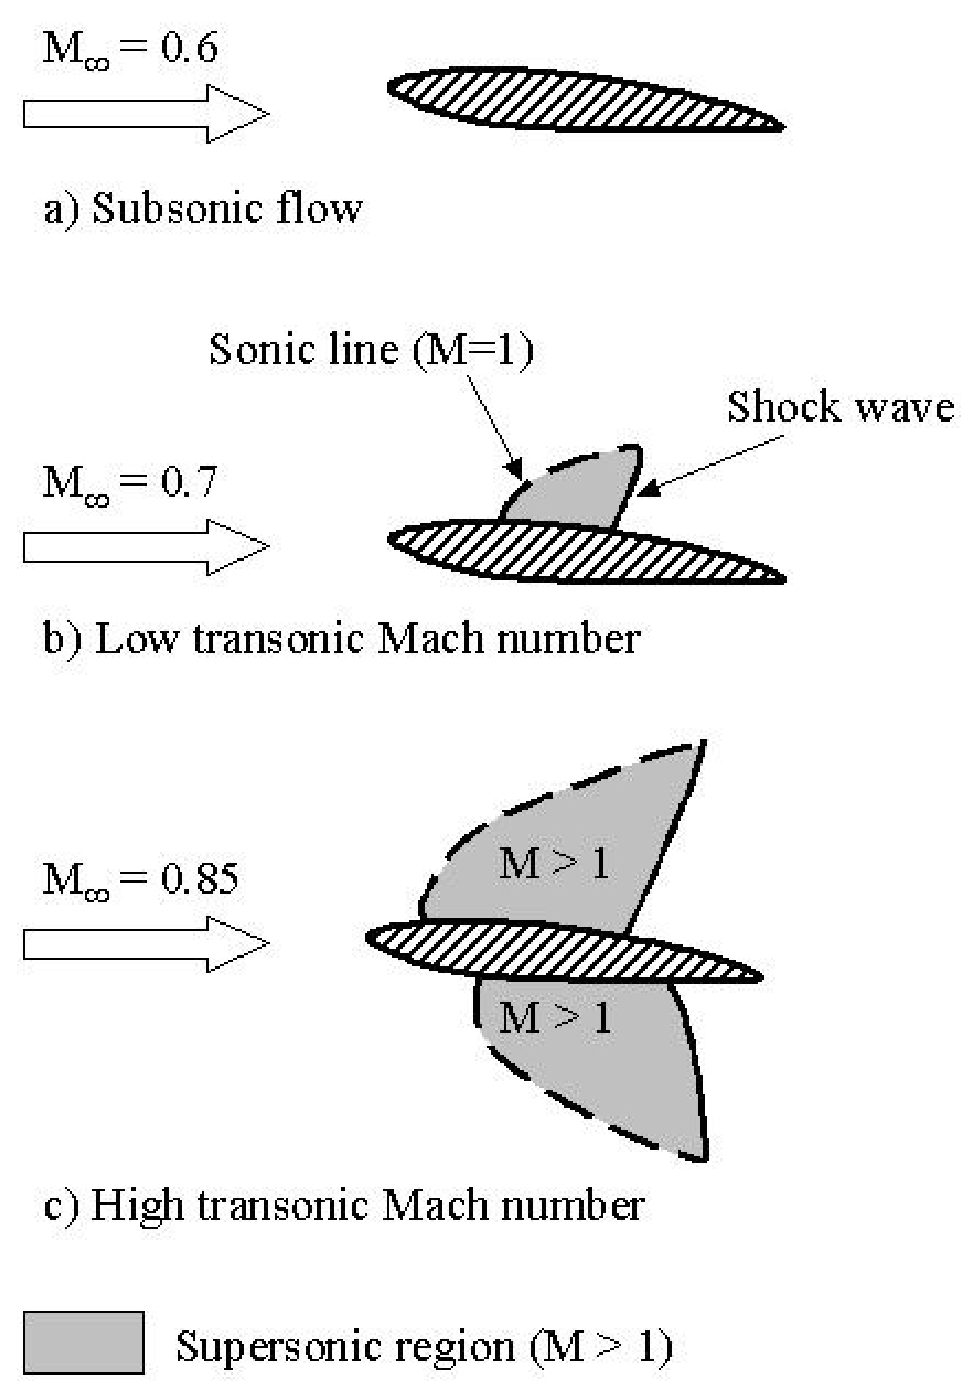
\includegraphics[height=6in]{aflow}
    \else
      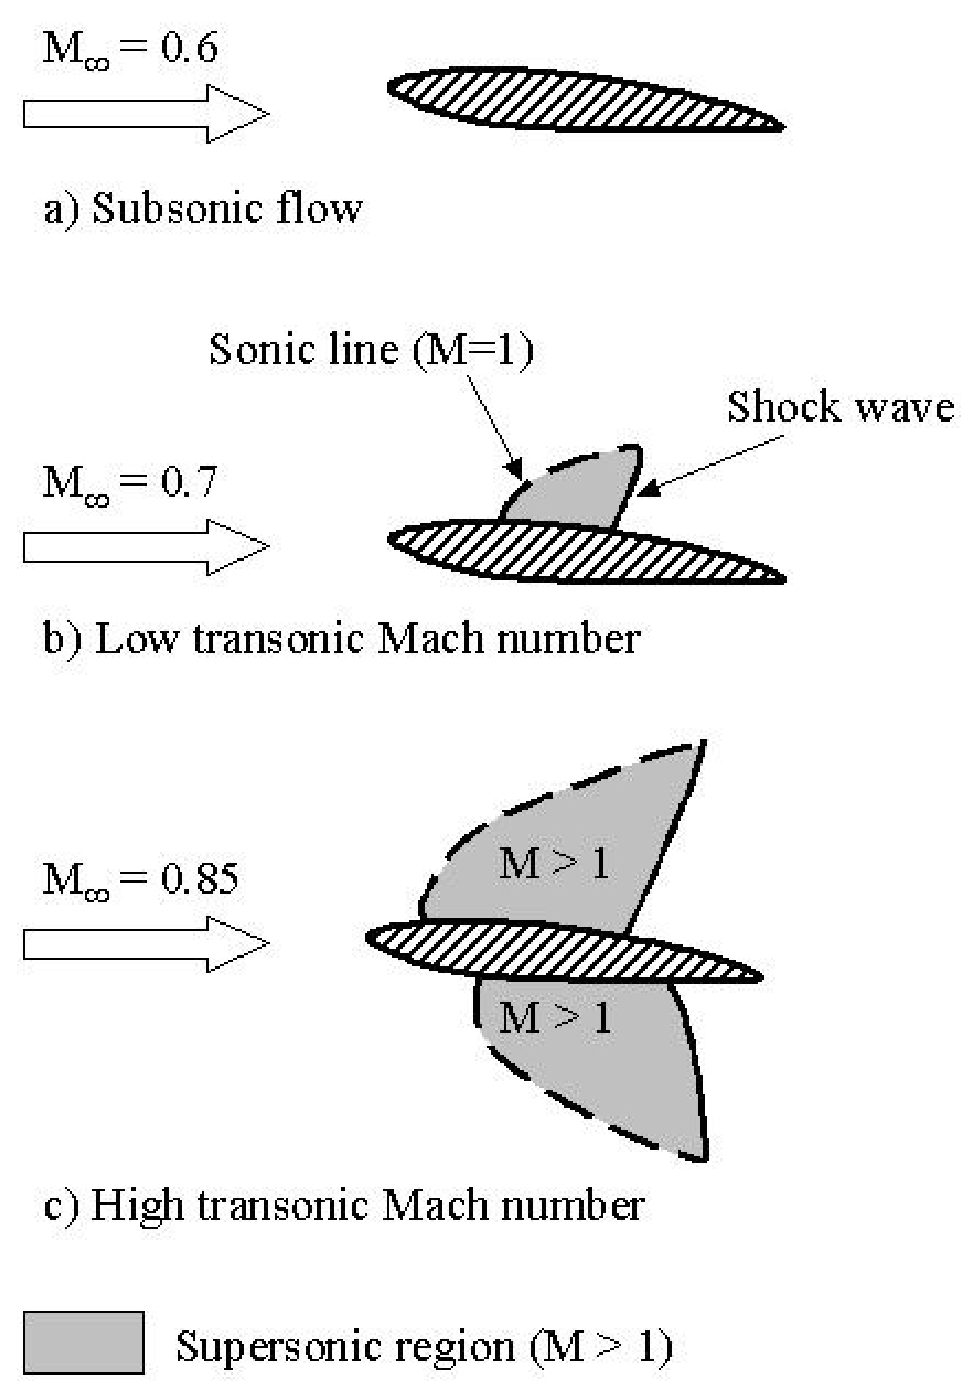
\includegraphics[bb = 92 86 545 742, height=6in]{aflow}
    \fi
    \caption{Airfoil Picture}
    \label{FigAir}
  \end{center}
\end{figure}

% above code has been macro-fied in Classes/MacroFile.tex file
%\InsertFig{\IncludeGraphicsH{aflow}{6in}{92 86 545 742}}{Airfoil Picture}{FigAir}

So as we have now labelled it we can reference it, like so Figure~(\ref{FigAir}) and it
is on Page \pageref{FigAir}. And as we can see, it is a very nice picture and we
can talk about it all we want and when we are tired we can move on to the next
chapter ...

I would also like to add an extra bookmark in acroread like so ...
\ifpdf
  \pdfbookmark[2]{bookmark text is here}{And this is what I want bookmarked}
\fi
\end{comment}
% ------------------------------------------------------------------------


%%% Local Variables: 
%%% mode: latex
%%% TeX-master: "../thesis"
%%% End: 
